\chapter{主播端的视频质量问题}
在这一章中,我们通过测量一些主流的个人直播应用,发现了主播端的质量下降问题。之后我们仔细分析了问题背后的原因,提出了可能的解决方案。

\section{主播端性能测量}
\begin{figure}[H]% use float package if you want it here
  \centering
  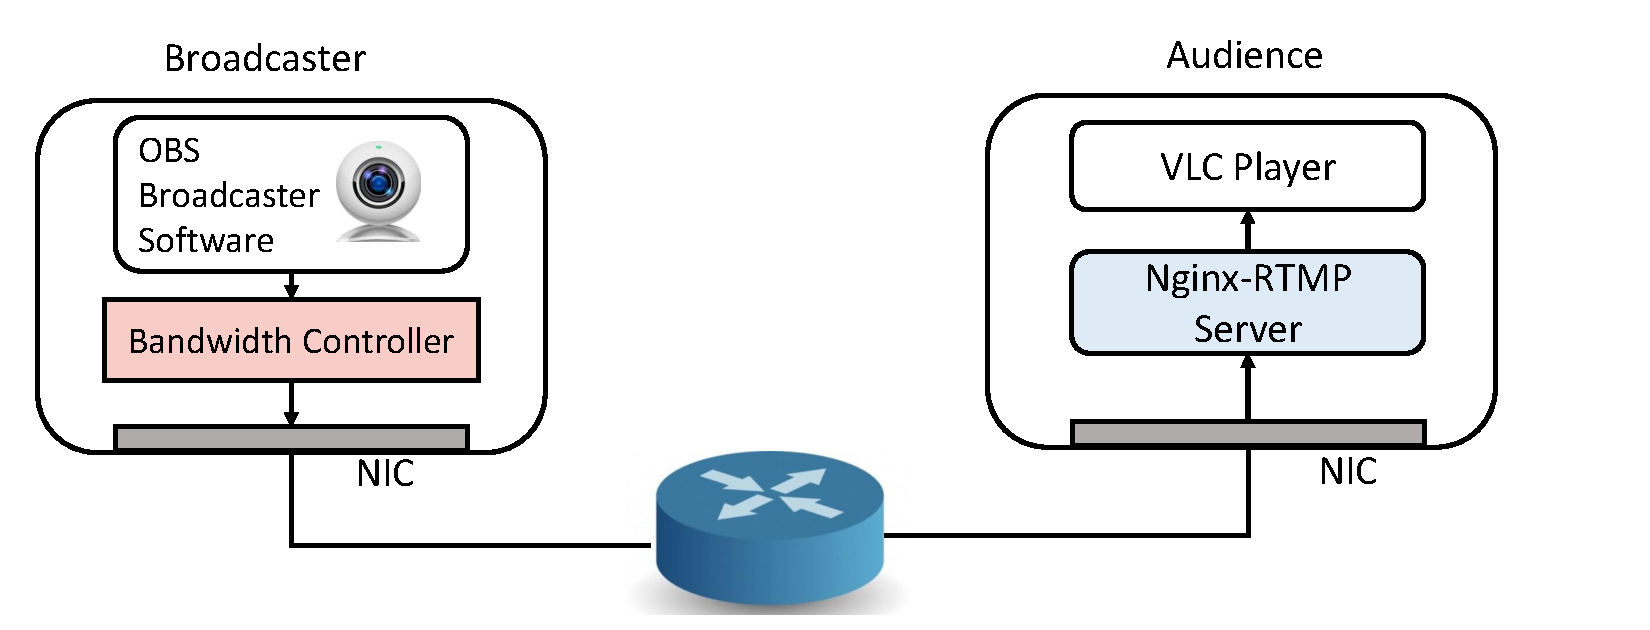
\includegraphics[width=\textwidth]{setup}
  \caption{实验设置}
  \label{fig:setup}
\end{figure}

\textbf{实验设置} 我们搭建了如图~\ref{fig:setup}所示的直播传输架构。 两端的设备(主播端和观众端)都有两个CPU核,6G内存,装备着100Mbps的网卡,他们通过中间的交换机连接在一起。主播端用OBS去发送视频,OBS是一个主流的使用RTMP协议的直播软件。另外,主播端有个带宽控制的模块,模拟无线环境的网络带宽变化。带宽控制模块是用Linux的tc模块和dummynet来实现的。观众端使用nginx-rtmp模块搭配rtmp接收服务器,接收视频,并用VLC播放器播放接收到的RTMP流。

\subsection{案例分析:变化带宽下性能不佳}
我们根据无线网络下的真实数据去控制网络带宽变化。数据记录的是当一个用户通过移动设备浏览亚马逊网站时的实时带宽。我们按照5秒的时间间隔去统计发送的总数据包数,然后计算每个时隙的总数据量。我们根据带宽的数据去控制主播端的网络带宽,数据记录的平均带宽大于3300kbps。 开始我们把码率设为3300kbps,用OBS去上传视频,并在观众端用tcpdump去抓取报文。结果如图~\ref{fig:case_study}所示。数据记录持续时间为320s,我们把记录分为两部分,0-140s以及120-260s。

\begin{figure}[h]
  \centering%
  \begin{subfigure}{0.7\textwidth}
    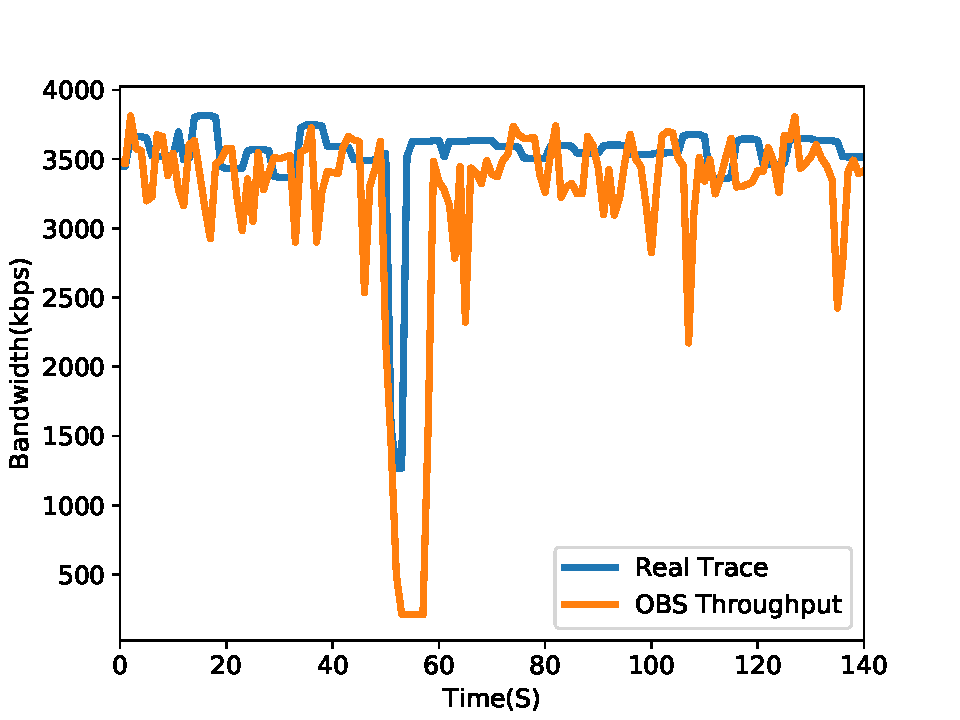
\includegraphics[width=\textwidth]{case_study_throughput_a}
    \caption{0-140s的吞吐量}
    \label{fig:case_study_a}
  \end{subfigure}%
  \vfill
  \vspace{0.2in}
  \begin{subfigure}{0.7\textwidth}
    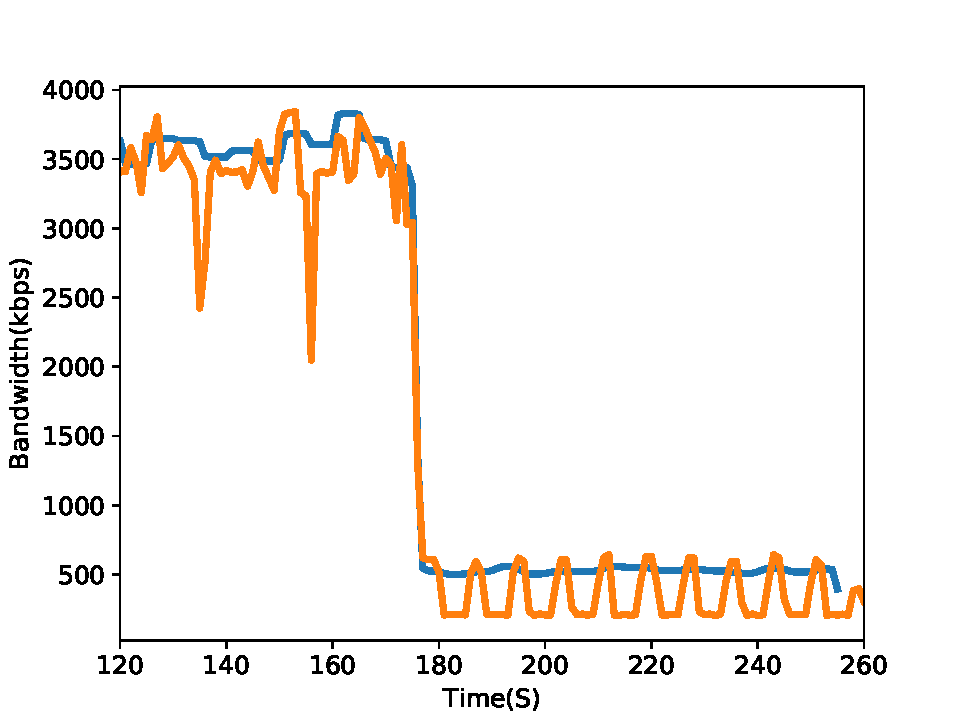
\includegraphics[width=\textwidth]{case_study_throughput_b}
    \caption{120-260s的吞吐量}
    \label{fig:case_study_b}
  \end{subfigure}
  \caption{无线网络环境下直播应用的吞吐量}
  \label{fig:case_study}
\end{figure}

从实验图,我们得出两个结论。(1)在图~\ref{fig:case_study_a}中,实际带宽紧紧跟随带宽数据变化,然而,在50s时,带宽下降到码率以下,这种情况维持了2s,然而真实的吞吐量降为0,维持了8s,从50s到58s。这是一种不正常的现象,2s的网络抖动导致了直播流8的吞吐量下降。(2)从图~\ref{fig:case_study_b}可以看出固定的码率不能有效的解决长时间的带宽变化。0-180s带宽是充足的,但是180s之后带宽急剧下降,这个过程持续了80s,在这期间发生了大量的丢帧。在这个很差的网络环境下,OBS算法依然默认设置之前的码率,这个策略显示不够令人满意。

\subsection{带宽波动普遍存在}
\begin{figure}[h]
  \centering%
  \begin{subfigure}{0.7\textwidth}
    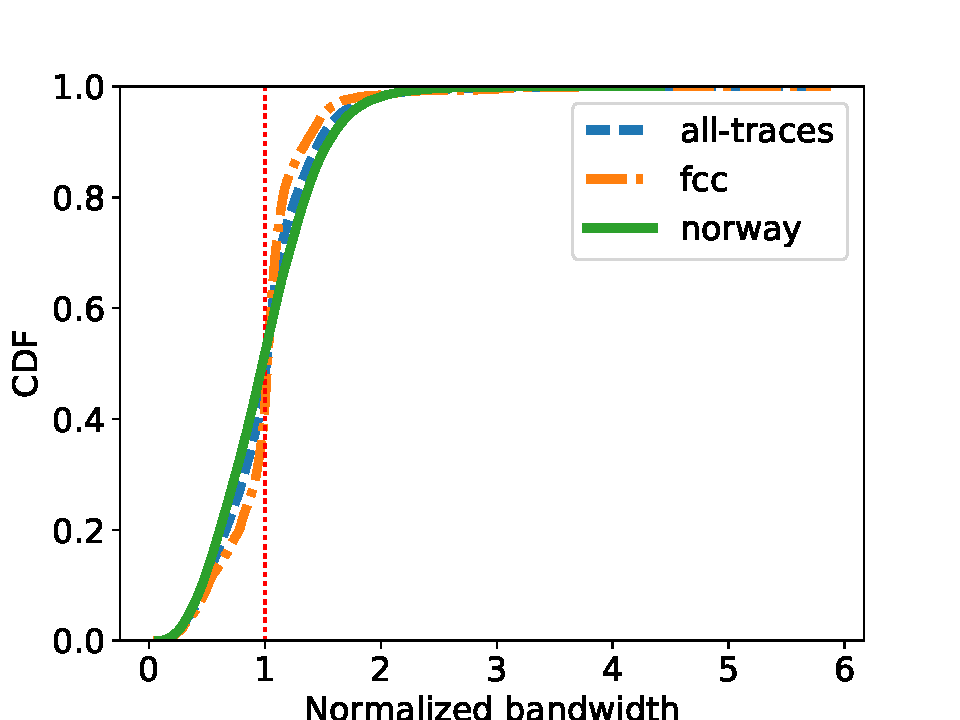
\includegraphics[width=\textwidth]{trace}
    \caption{归一化带宽累计分布函数}
    \label{fig:trace}
  \end{subfigure}%
  \vfill
  \vspace{0.2in}
  \begin{subfigure}{0.7\textwidth}
    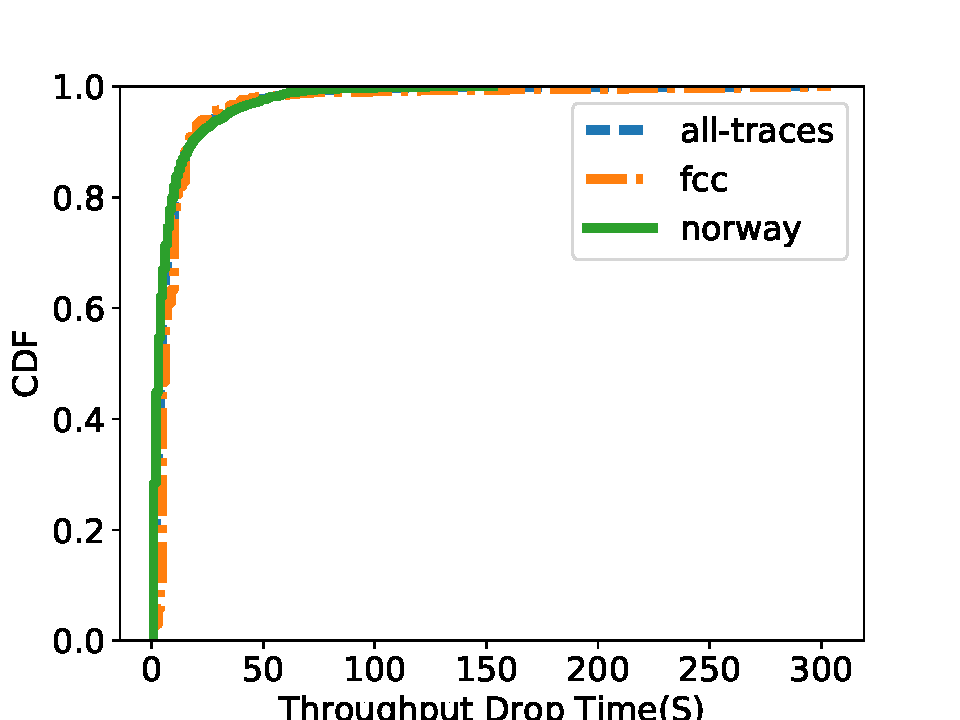
\includegraphics[width=\textwidth]{trace-down}
    \caption{带宽抖动时长分布}
    \label{fig:trace_down}
  \end{subfigure}
  \caption{无线网络环境的带宽分布}
  \label{fig:case_study}
\end{figure}

我们通过分析两个真实数据集的带宽分布来预估带宽抖动发生的频率。两个数据集分别是FCC数据集和HSDPA数据集,每个记录持续320s,数据集共持续了30多小时。对于每一个记录来说,我们根据平均带宽去归一化记录,画出了它的cdf图~\ref{fig:trace}。50\%左右的记录在平均带宽以下,这意味着对于一个10s的带宽记录来说,有5s的时间,带宽会低于平均值。20\%的记录只有平均值的一半。该图表明在现实世界的网络中,带宽波动频繁发生。为了进一步说明带宽抖动持续的时长,我们画了一张带宽抖动时长分布的图~\ref{fig:trace_down}。带宽抖动时长等于带宽在平均值以下的持续时间。大约20\%的网络抖动持续时长多于10s,有些甚至持续数百秒。另外,我们还可以从上面的两个图中看出,FCC数据集和HSDPA数据集的分布和整体类似。

\subsection{商业平台验证}

\begin{figure}[htb]
  \centering%
  \begin{subfigure}{\textwidth}
    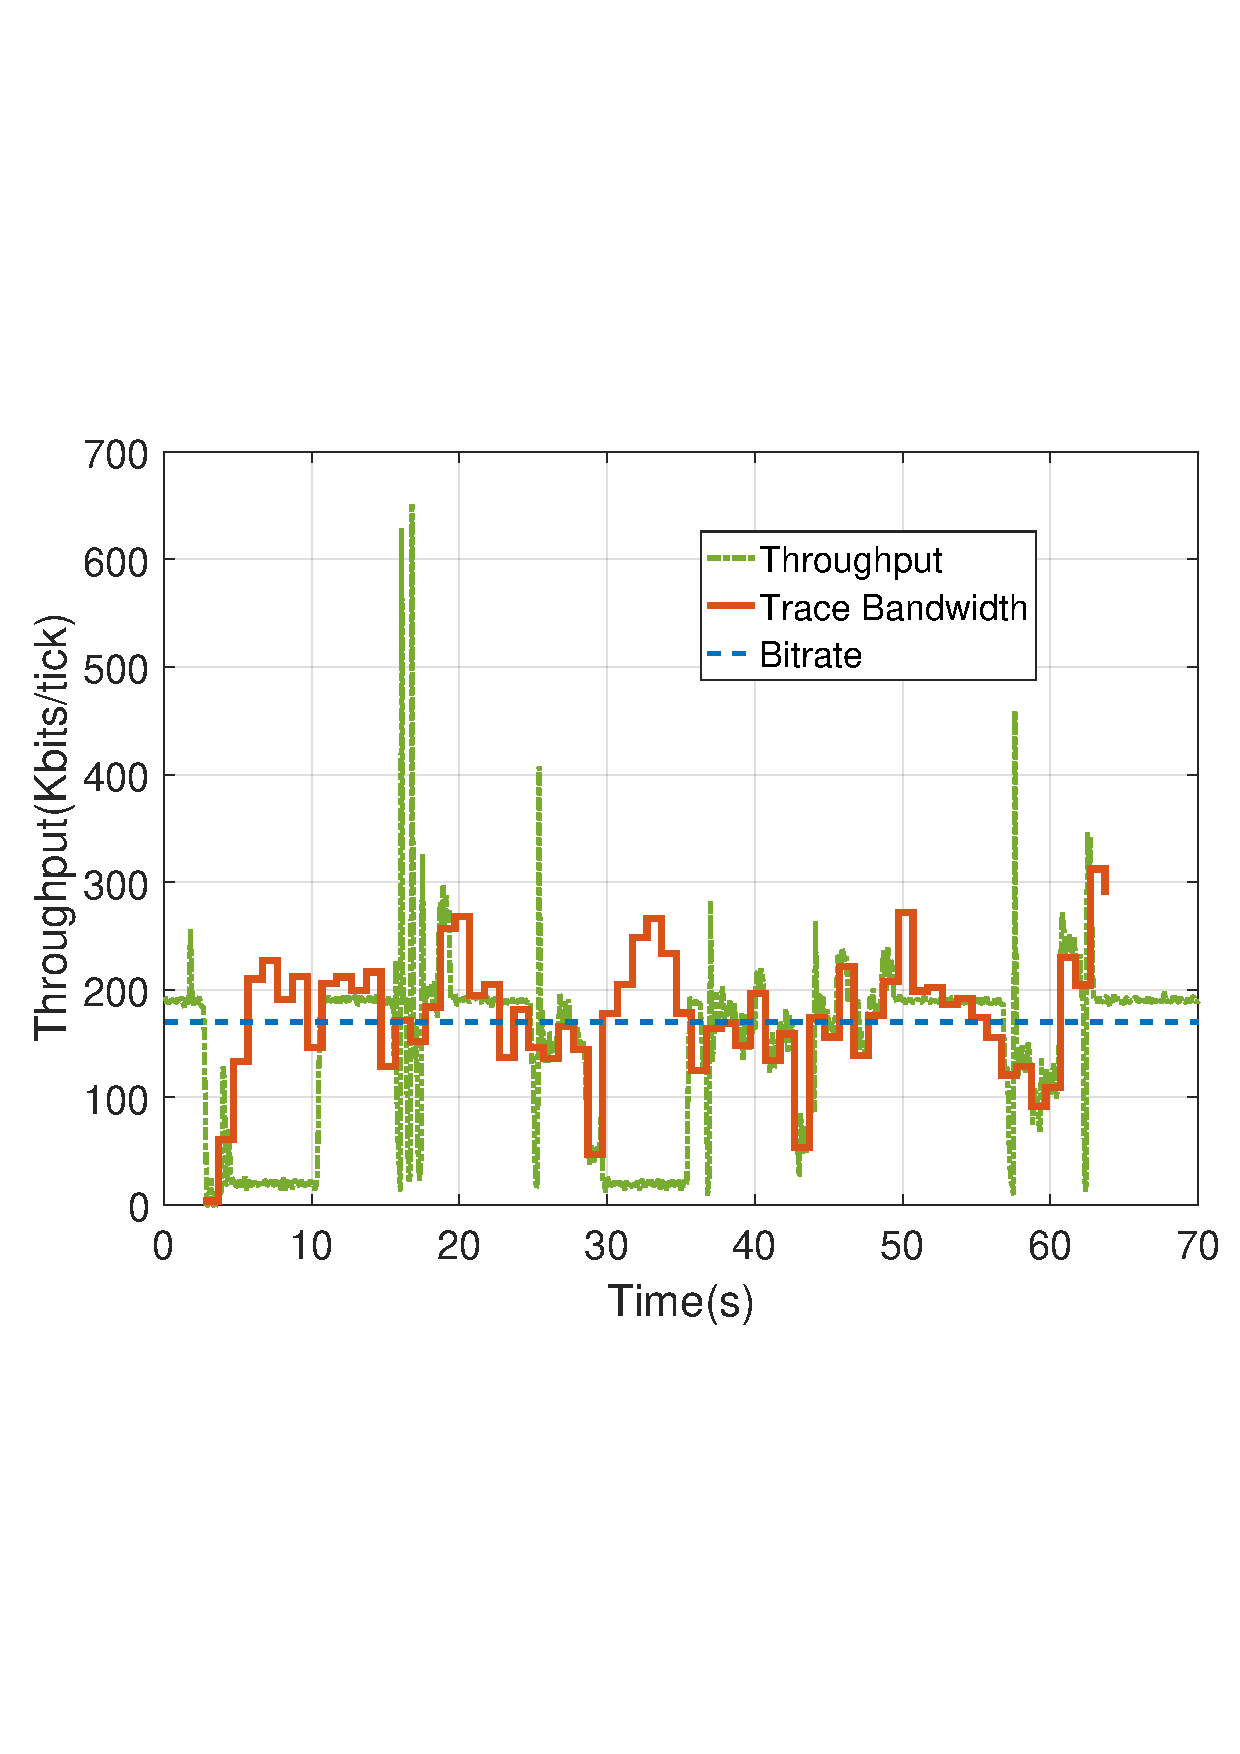
\includegraphics[width=0.5\textwidth]{obs_douyu}
    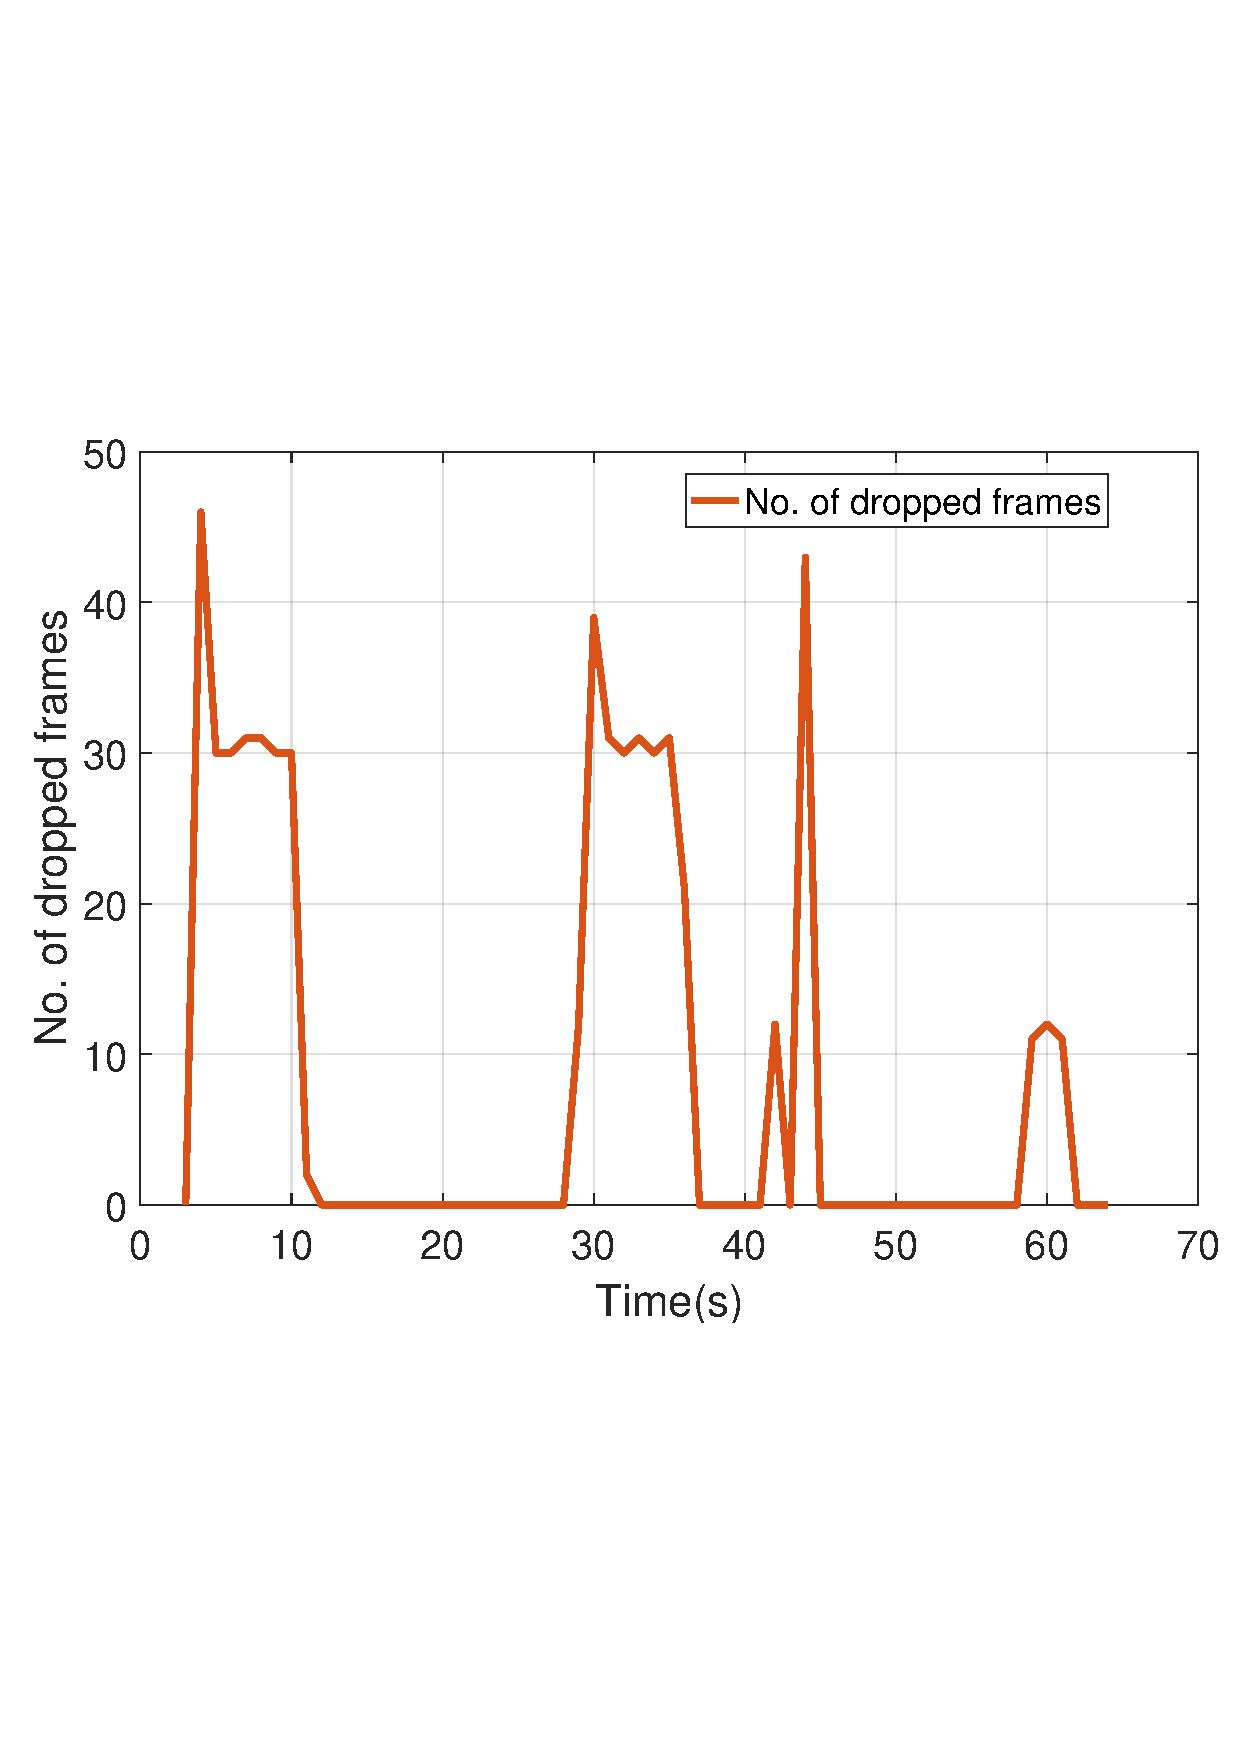
\includegraphics[width=0.5\textwidth]{obs_douyu_drop}
    \caption{OBS推流至斗鱼服务器的吞吐量和丢帧}
    \label{fig:obs_douyu}
  \end{subfigure}%
  \vfill
  \vspace{0.2in}
  \begin{subfigure}{\textwidth}
    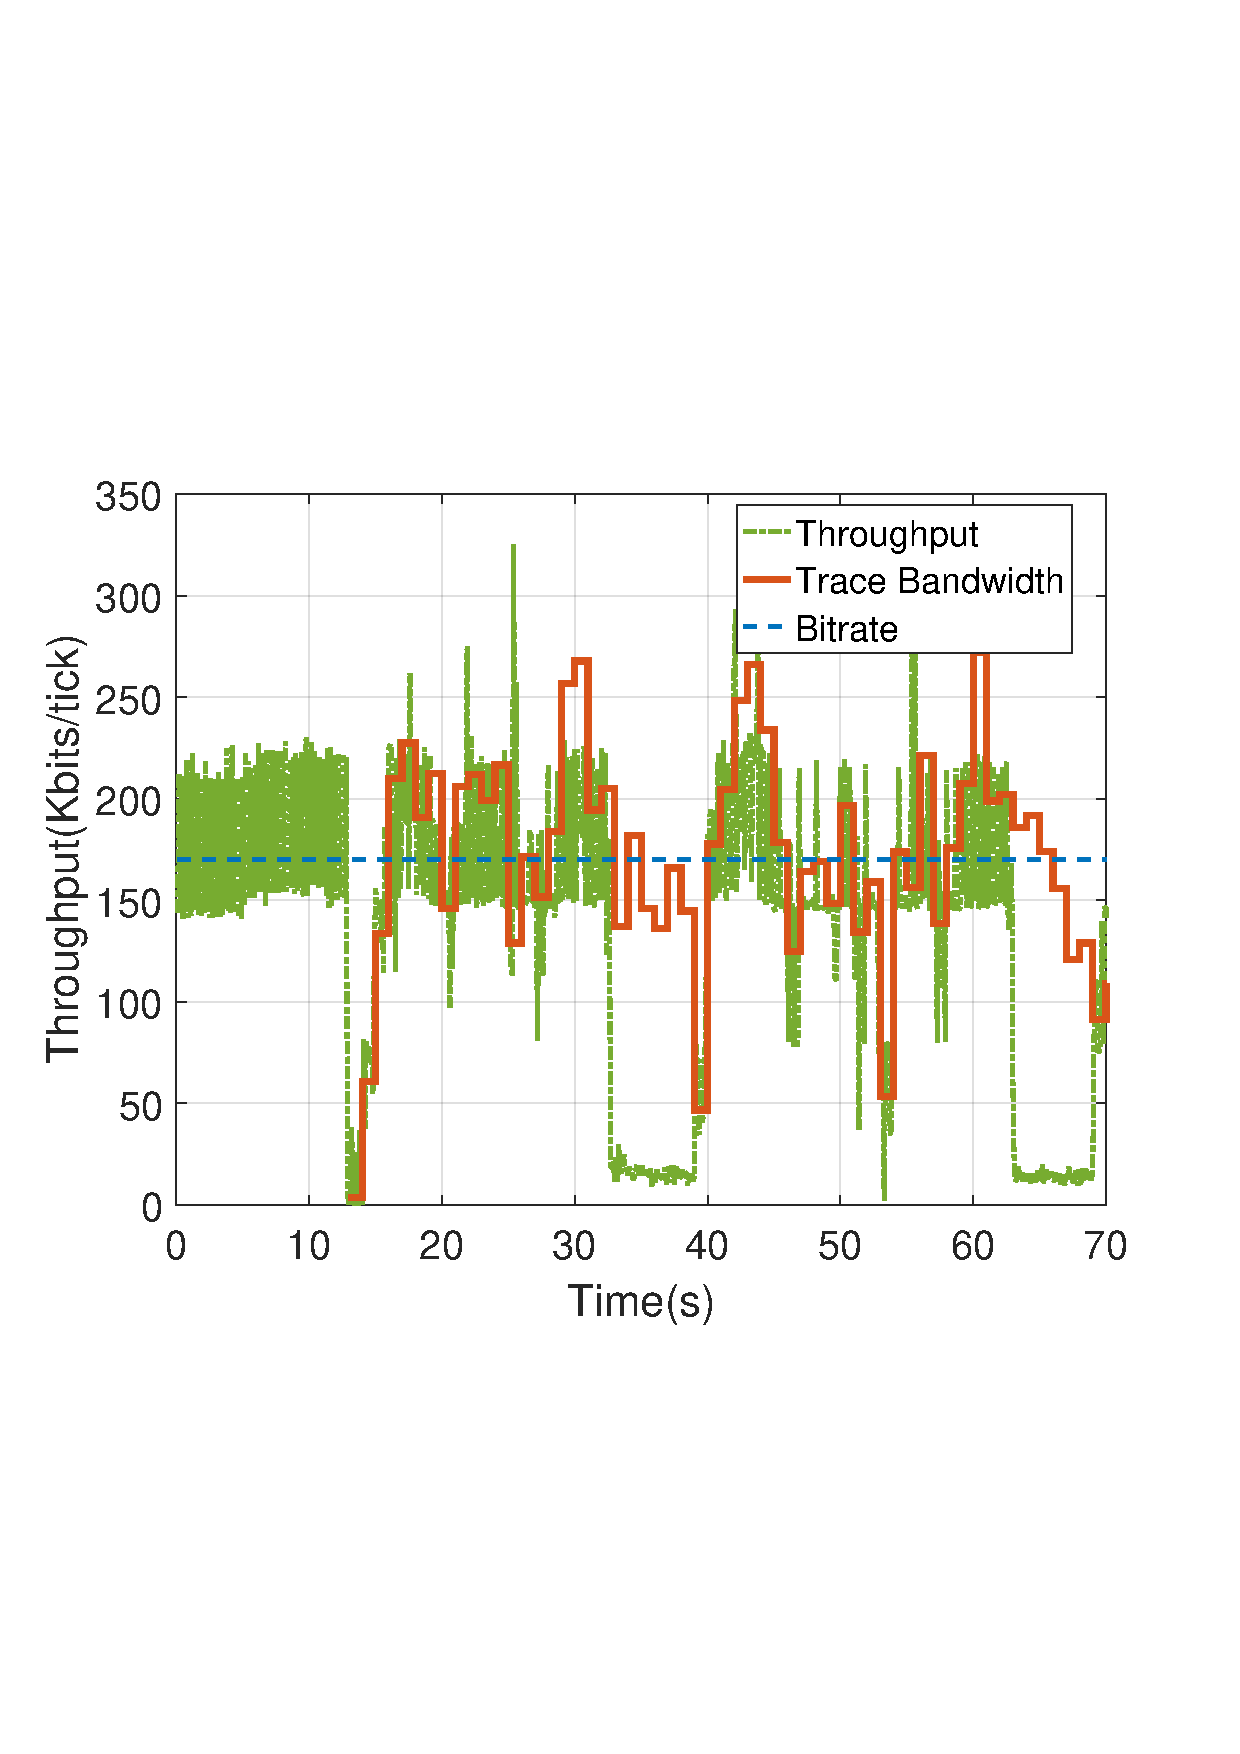
\includegraphics[width=0.5\textwidth]{douyu}
    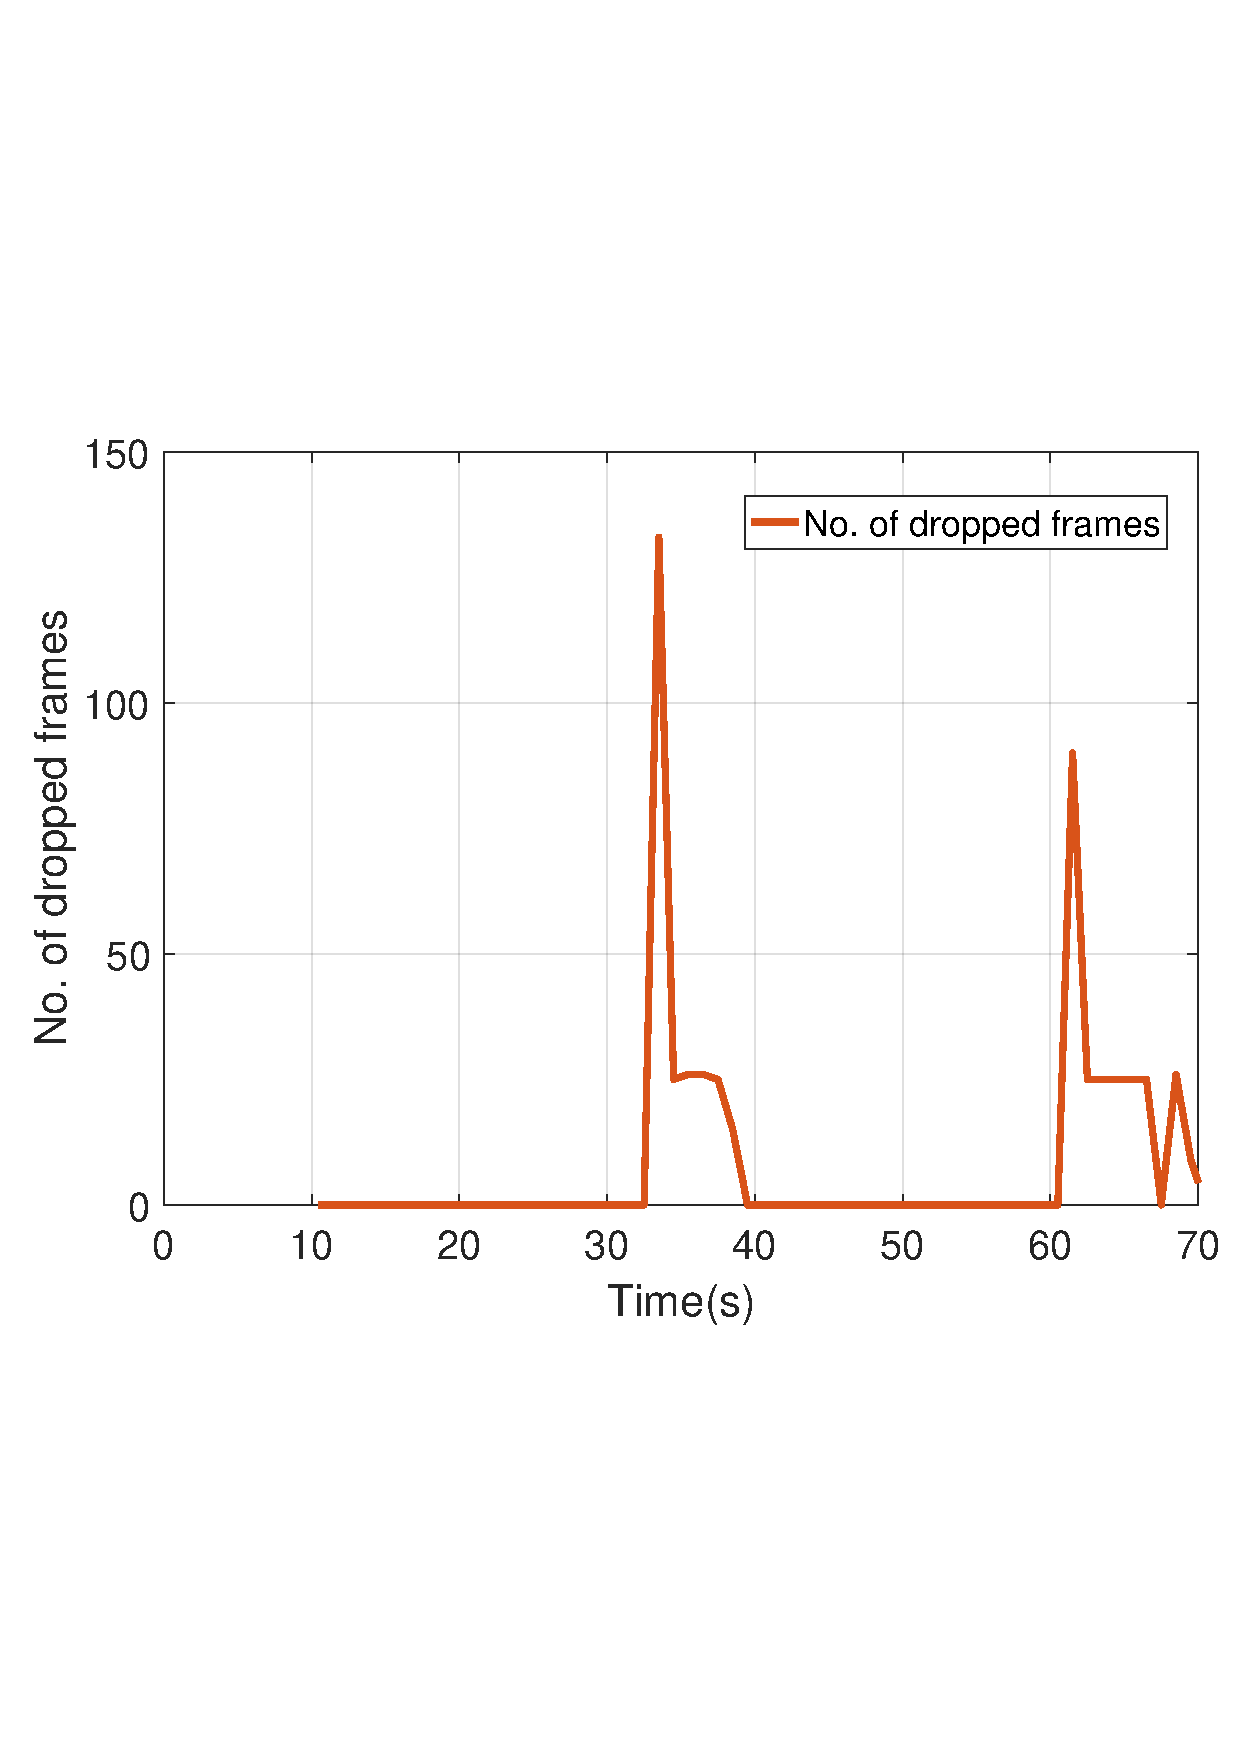
\includegraphics[width=0.5\textwidth]{douyu_drop}
    \caption{斗鱼主播工具推流至斗鱼服务器的吞吐量和丢帧}
    \label{fig:douyu}
  \end{subfigure}
  \vfill
  \vspace{0.2in}
  \begin{subfigure}{\textwidth}
    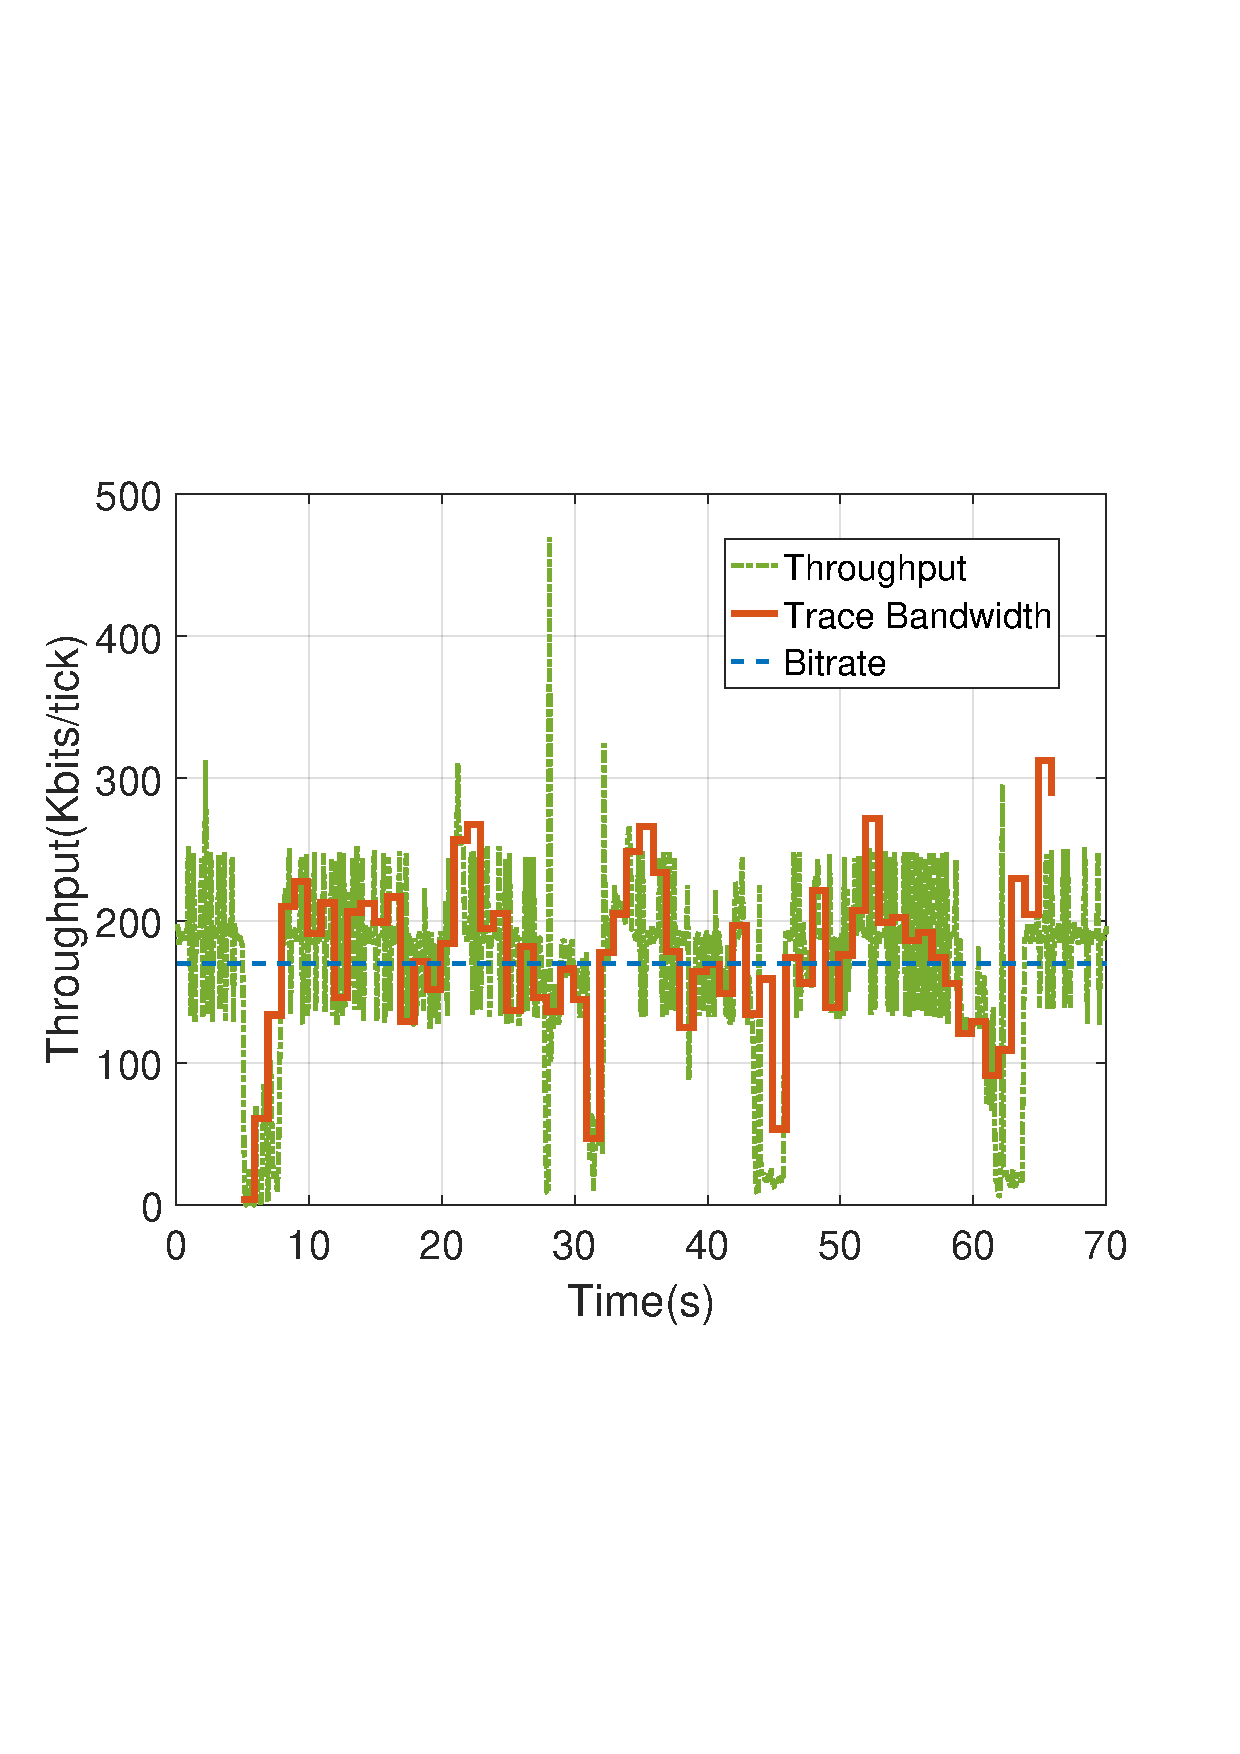
\includegraphics[width=0.5\textwidth]{obs_twitch}
    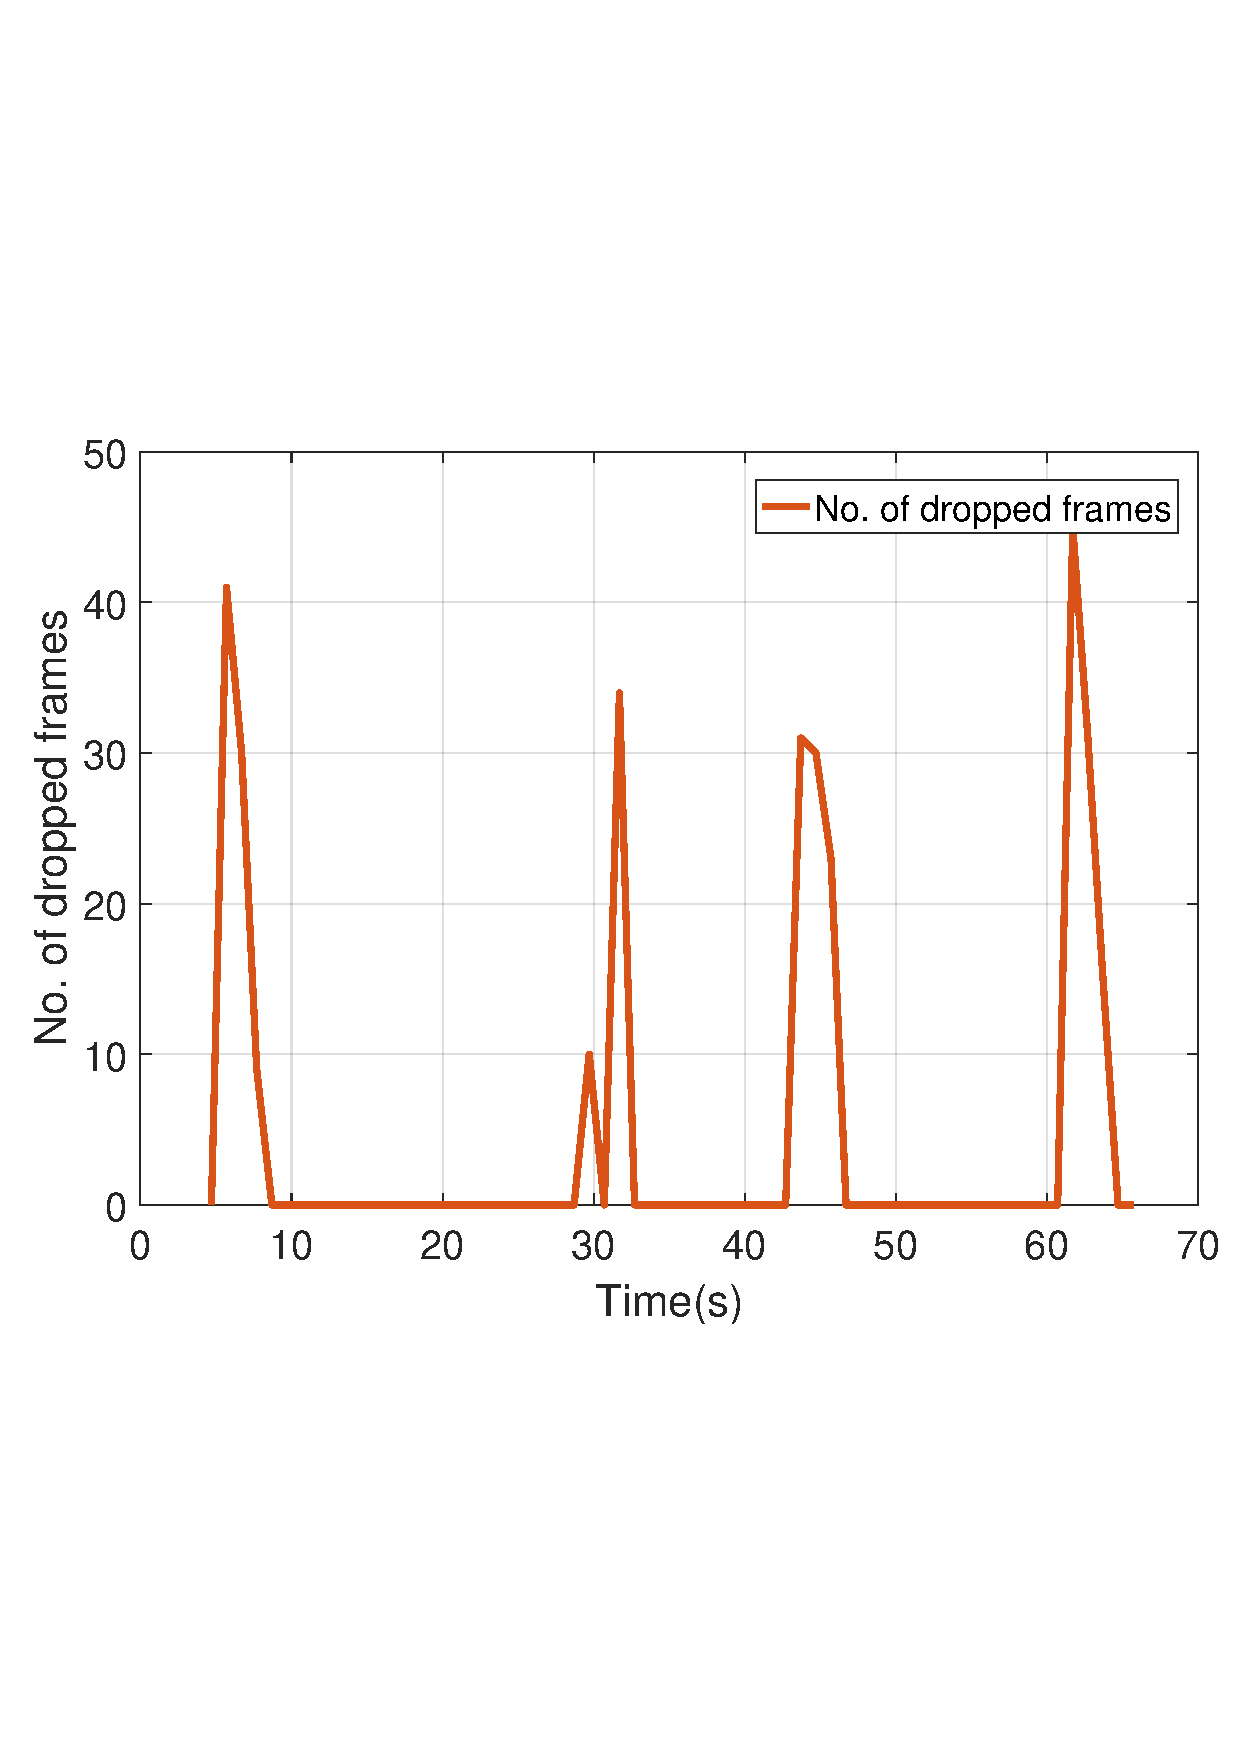
\includegraphics[width=0.5\textwidth]{obs_twitch_drop}
    \caption{OBS推流至Twitch服务器的吞吐量和丢帧}
    \label{fig:twitch}
  \end{subfigure}
  \caption{商业平台验证实验}
  \label{fig:commerical_application}
\end{figure}

为了验证商业平台上是否存在相同的问题,我们选择了几个交互直播的商业组合去重复上述实验。分别是OBS作为主播端推流到斗鱼服务器,斗鱼主播工具推流到斗鱼源服务器,OBS推流到Twitch的服务器。在三个实验中,平均可用的带宽高于初始码率1700kbps,然后在过程中带宽会偶尔低于初始码率。我们用TCPDUMP去记录真实的带宽。图~\ref{fig:commerical_application}分别表示了三个配置带宽和真实吞吐量的时序图,以及丢帧数的时序图。表~\ref{tb:drop}的前三行总结了每个实验中总的丢帧数。

\begin{table}[htb]
\centering
\caption{不同实验配置下的丢帧数}
\label{tb:drop}
{\setlength{\tabcolsep}{2pt}
\begin{tabular}{|c|c|c|l|}
\hline
\textbf{实验组} & \textbf{实验配置} & \textbf{上传失败时长} & \textbf{失败比例(\%)}   \\ \hline
\multirow{3}{*}{Figure ~\ref{fig:commerical_application}}&  Obs-douyu               & 18.1         & 30.2\%                           \\ \cline{2-4}
& Obs-twitch              & 9.9        & 16.3\%    \\ \cline{2-4}
& Douyu-douyu            & 16.6      & 27.2\% \\ \hline
\multirow{4}{*}{Figure 7} & Obs-douyu            & 93.1      & 37.2\%     \\ \cline{2-4}
& Obs-twich             & 79.3      & 31.7\%  \\ \cline{2-4}
& Douyu-douyu             & 66.67         & 26.7\%  \\ \hline
\end{tabular}}
\end{table}

对比不同平台下的结果,我们发现放大效应很普遍,所有的平台都出现了这个问题(OBS推流至斗鱼的情况下出现在30-36s,斗鱼主播工具推流时发生在32-39s,推流至Twitch时出现在43-45s)。在三个时间段内,丢帧数一直保持一个很高的值。另外,我们发现级联效应的出现和带宽下降的幅度关系没有必然联系。例如,图5中,30s带宽剧烈下降,导致了级联效应。但在图b中,32s时轻微的带宽降低也导致了丢帧。另外一个发现是,级联效应导致的丢帧时长在不同平台上不同:斗鱼平台会有多于5秒的丢帧,Twitch平台上只有2-3s。总之,上述的实验结果表明商业平台的直播端依然不能有效的解决短时间的带宽下降。

\begin{figure}[H]% use float package if you want it here
  \centering
  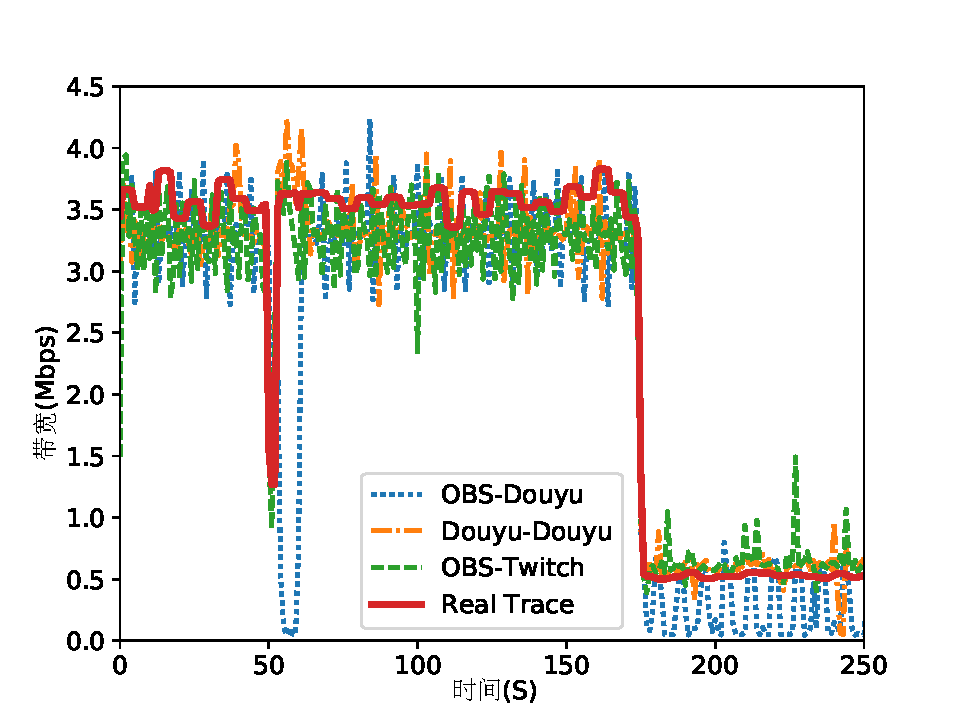
\includegraphics[width=\textwidth]{vary-bandwidth}
  \caption{长时间带宽抖动状况下的吞吐量}
  \label{fig:vary-bandwidth}
\end{figure}

我们还验证了长时间带宽下降时商业平台的性能表现,如图~\ref{fig:vary-bandwidth}所示。180s之后带宽剧烈下降,在这期间我们持续观察码率,发现所有三个实验的码率保持不变,均为初始码率。码率大于带宽,视频数据产生的速度远远大于网络容量。OBS推流至斗鱼服务器性能最差,而且没有充分利用带宽,其他的情况跟随带宽变化,但过程中一直持续不断的丢帧。表2记录了丢帧的数据。总的来说,现有的商业平台不能有效解决长时间带宽下降的情境下丢帧的问题。

\section{追溯根本原因}

\begin{figure}[H]% use float package if you want it here
  \centering
  
\includegraphics[width=\textwidth]{drop}
  \caption{视频帧队列示意图}
  \label{fig:drop}
\end{figure}

为了应对带宽抖动,主播端应该会有个队列存储视频帧。视频帧队列的示意图如图~\ref{fig:drop}所所示。摄像头抓取画面,之后将原始画面编码成H264格式的帧,之后把编码完的帧放入队列。同时发送进程从队列中取出一个视频帧,并将它通过TCP的socket端口发送到网络中去。如果网络状况不好,帧发送的进程会被堵塞,队列由于超出空间限制发生溢出,新产生的视频帧不再纳入队列,于是发生了丢帧。

\begin{figure}
\centering
%\small
{\setlength{\tabcolsep}{3pt}
\begin{tabular}{|r||ccccccccc|cc|}
\hline
帧类型       & I & B & B & P & B & B & P & B & B  & I  & ... \\ \hline
播放顺序   & 1 & 2 & 3 & 4 & 5 & 6 & 7 & 8 & 9  & 10 & ... \\ \hline
编码顺序 & 1 & 3 & 4 & 2 & 6 & 7 & 5 & 9 & 10 & 8  & ... \\
\hline
\end{tabular}}
\caption{H.264帧的编码顺序和播放顺序}
\label{fig:frame-order}
\end{figure}

短时间的带宽抖动导致的丢帧级联效应主要是由于帧之间存在依赖性。在H264中,一段视频会被编码成一组图片,称为一个GoP。编码时,一组图片的第一帧应保持不变,这一帧称为I帧。P帧是通过计算与上一个I帧或者P帧的差值生成的;B帧根据邻近的I帧和P帧产生。表~\ref{fig:frame-order}给出了一系列连续的帧的示意图,按照播放顺序展示。但解码和编码的顺序和播放的顺序并不一样。因为帧之间的依赖关系,当一组GoP中间的P帧被丢弃,之后所有的P帧和B帧都不能够解码。因此,如果网络中一个小抖动导致GoP的中间或者开头出现丢帧,级联效应会导致剩余的帧都不能解码,或者丢掉。

\begin{algorithm}[htb]
\caption{OBS默认丢帧算法}
\label{alg:obs-drop}
{\bf Require:}timespan:队列时间跨度;dropPFrame:P帧相关的丢帧优先级;dropBFrame:B帧相关的丢帧优先级;bandwidth:每一时刻的带宽
\begin{algorithmic}[1]
\State T1 := 0.9秒,T2:=0.7秒,timespan :=0
\If{新产生的帧是I帧}
\State dropPFrame := False, dropBFrame :=False
\State \Call{入队}{视频帧队列, 新产生的帧}
\State timespan:= timespan + 1
\EndIf
\If{新产生的帧是P帧}
\If{dropPFrame or timespan $>$ T1}
\State \Call{丢弃}{新产生的帧},丢弃所有的I帧和P帧
\State timespane := timespan - 丢弃的时长
\Else
\State \Call{入队}{视频帧队列, 新产生的帧}
\State timespan := timespan + 1
\EndIf
\EndIf
\If{新产生的帧是B帧}
\If{dropBFrame or timespan $>$ T2}
\State \Call{丢弃}{新产生的帧},丢弃所有的B帧
\State timespan := timespan - 丢弃的时长
\Else
\State \Call{入队}{视频帧队列,新产生的帧}
\State timespan := timespan + 1
\EndIf
\EndIf
\State timespan := timespan - \Call{发送的时长}{bandwidth}
\end{algorithmic}
\end{algorithm}


我们通过分析OBS主播软件的源码,研究了它的队列管理算法,如图算法~\ref{alg:obs-drop}。算法引入了两个变量,丢帧优先级和队列时间跨度。丢帧优先级是为了避免对无法解码的帧的无效传输,队列时间跨度表示队列中最旧的帧和当前时间的差值。当丢帧发生时,优先级被置为True,视频队列停止接收GoP中其余的帧。一开始,丢帧优先级会被初始化为False。当一个新的帧产生时,先判断是否是I帧,如果是,入队,将所有的丢帧优先级赋值为False。否则,计算队列中最老的帧和当时间的差值,赋值给队列时间跨度。如果产生的帧是p帧,同时时间跨度小于0.9s,则P帧入队。如果P帧对应的优先级为True,则丢弃当前帧;或者如果时间跨度多余0.9s,丢弃队列里所有的P帧和B帧,包括当前GoP未产生的那些帧。B帧和P帧的丢帧优先级都被设为True。如果新产生的帧是B帧,决定是否的阈值是0.7s,其余的逻辑和P帧类似。

对于长时间的带宽抖动,我们通过上述的实验观察到,主播端的码率一直保持为初始的码率,视频数据产生的码率远远大于可用的无线带宽,就会发生丢帧。在这个过程中,如果GoP中靠前的P帧或者I帧被丢弃,那么级联效应会导致性能进一步恶化。问题存在的根本原因是视频码率不能根据瞬时的带宽调节。

\section{优化空间}
丢帧问题明显降低了视频质量,但是简单的解决方案,比如增加视频队列的长度违反了及时性的要求。因此,在我们的解决方案中,为了满足及时性要求,我们保持视频队列长度足够小。我们提出了视频帧产生和传输的机制去改善视频质量,适应变化的带宽。我们把视频队列的空间大小限制在0.9s以内。前面的实验给了我们改善视频传输质量的几个方向。

\begin{description}
  \item[减小帧之间的依赖性] 帧之间的依赖性由于H264的视频压缩算法导致,非关键帧都是由关键帧计算得来。关键帧之间是相互独立的,依赖性只存在在一个GoP内部。减小帧之间依赖性的一个直接的做法就是减少关键帧间隔。举个最极端的例子,如果关键帧间隔为1帧,那么帧之间完全不存在依赖性。另外,假设在关键帧为8s的情况下,如果在一个GoP开始时,发生了一个2s的网络抖动,那么整个GoP都会被丢弃;但是如果8s的关键帧间隔被修改为2s,就只会丢弃一个2s的GoP。这样修改,级联效应被弱化了。然而,这个方法需要在最小化帧间隔和视频质量之间达到一个平衡。因为减少关键帧间隔意味着减少对画面的压缩,为了维持设定的码率,每帧画面的质量都有所降低,甚至出现大的像素块。
  \item[智能的丢帧策略] OBS默认的策略是当队列时间跨度超出阈值后丢帧队列里所有的P帧和B帧。算法现在的设计有一定的理由,因为如果丢弃队列中较老的帧,剩余的帧也就无法解码。但是如果丢弃最新的视频,老的视频帧依然存在在队列中,及时性无法保证。但是,对于队列中同时存在2个或者多个GoP的情况,一个直接的可以优化的点就是,丢弃旧的GoP的帧。这样的方法相对于OBS的默认策略会有一定的提升。设计出一个接近最优解决方案的在线的丢帧策略很重要,唯一的挑战在于帧之间存在依赖性。暴力搜索方式虽然可以找出最优解,但是由于时间复杂度太高,所以实际中并不可用。
  \item[自适应码率] 图4说明了网络带宽抖动频繁发生,之前的测量显示商业平台只使用固定码率或者平均码率的方式去编码视频。平均码率的方式是指实际的带宽可以在目标码率附近波动。这两种编码方式都不能动态跟随带宽变化,当带宽下降时,会发生大量的丢帧。如果带宽降低持续时长较长的话,这种现象尤其明显。一个可能的解决方案是类似于点播情况下的DASH,在主播端动态改变码率。我们的选择是以GoP的级别去改变码率,为每一个GoP选择一个码率。引入码率自适应的方式可能会大幅度的减少丢帧。
\end{description}
